\chapter{Introduction}
\label{chapter:introduction}


\section{The problem of clustering}
\label{sec:clustering}

%this is mostly taken from Jain's 50 years beyond K-Means
Advances in technology allow for the collection and storage unprecedented amount and variety of data. Since data is mostly stored electronically, it presents a potential for automatic analysis and thus creation of information and knowledge. A growing body of statistical methods aiming to model, structure and/or classify data already exist, e.g. linear regression, principal component analysis, cluster analysis, support vector machines, neural networks. Many of these methods fall into the realm of machine learning, which is usually divided into 2 major groups: \textit{supervised} and \textit{unsupervised} learning.
% (explain what learning is) The task of learning is...
Supervised learning deals with labelled data, i.e. data for which ground truth is known, and tries to solve the problem of classification. Unsupervised learning deals with unlabelled data and tries to solve the problem of clustering.

Cluster analysis is the backbone of the present work.
The goal of data clustering, as defined by \citep{Jain2010}, is the discovery of the \textit{natural grouping(s)} of a set of patterns, points or objects. In other words, the goal of data clustering is to discover structure on data, structured or not.
And the methodology used is to group patterns that are similar by some metric (e.g. euclidean distance, Pearson correlation) and separate those that are dissimilar. %TODO reference for a method for both euclidean distance and Pearson correlation

As an example, Figure \ref{fig:intro raw} shows the plot of a simple synthetic dataset - a Gaussian mixture of 5 distributions.
No extra information other than the position of the points is given, since clustering algorithms are unsupervised methods.
Figure \ref{fig:intro natural} presents the desired (or "natural") clustering for this given dataset.
Figure \ref{fig:intro kmeans} presents the clusters given by the K-Means algorithm with an initialization of 4 clusters.
The number of clusters was purposefully set to an "incorrect" number to demonstrate that the number of cluster of a dataset is not trivial to discover, even in suck a simple example. In this synthetic dataset, the number of clusters is not clear due to the two superimposed Gaussians.

The number of clusters is a common initialization parameter for clustering methods.
When no prior information about the dataset is given, the number of clusters can be hard to discover.

%TODO change this 3 plots to a three plot subfigure, with the plots side by side
\begin{figure}[hbtp]
\centering
\includegraphics[scale=0.5]{introduction/img/cluster_example_raw.png}
\caption{Gaussian mixture of 5 distributions. The middle "ball" of points is 2 Gaussians that intersect.}
\label{fig:intro raw}
\end{figure}

\begin{figure}[hbtp]
\centering
\includegraphics[scale=0.5]{introduction/img/cluster_example_natural.png}
\caption{Gaussian mixture of 5 distributions. The colors of each point represents the group (the Gaussian distribution) to which it belongs.}
\label{fig:intro natural}
\end{figure}

\begin{figure}[hbtp]
\centering
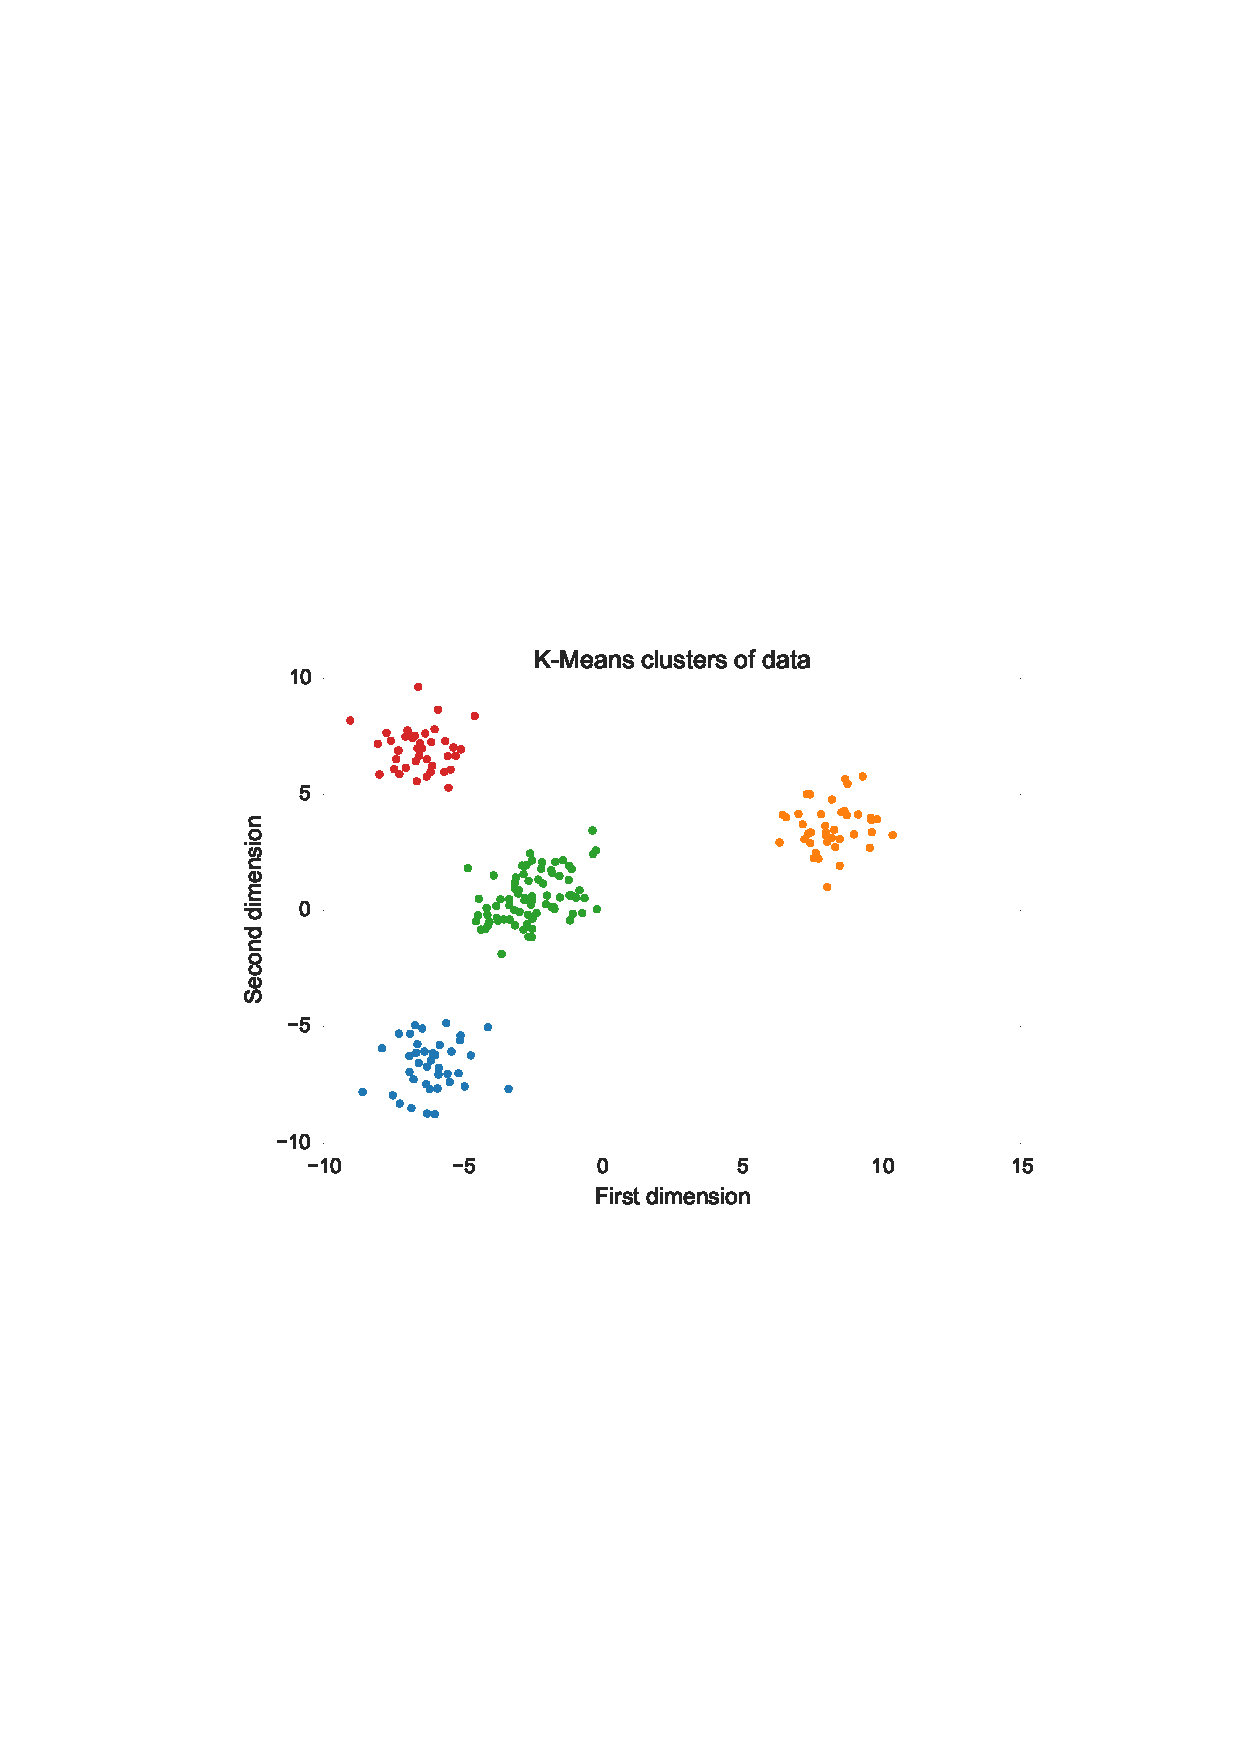
\includegraphics[scale=0.5]{introduction/img/cluster_example_kmeans.png}
\caption{Sama data, as Figure \ref{fig:intro raw}, but the group to which each point belongs to was computed by the K-Means algorithm with the number of clusters set to 4.}
\label{fig:intro kmeans}
\end{figure}

% \begin{figure}
% \begin{subfigure}{.5\textwidth}
%   \centering
%   \includegraphics[width=.8\linewidth]{introduction/img/cluster_example_raw.png}
%   \caption{1a}
%   \label{fig:sfig1}
% \end{subfigure}%
% \begin{subfigure}{.5\textwidth}
%   \centering
%   \includegraphics[width=.8\linewidth]{introduction/img/cluster_example_natural.png}
%   \caption{1b}
%   \label{fig:sfig2}
% \end{subfigure}
% \caption{plots of....}
% \label{fig:intro2}
% \end{figure}
% \end{document}

% \begin{figure}
%     \centering
%     \begin{subfigure}[b]{0.3\textwidth}
%         \centering
%         \includegraphics[width=\textwidth]{introduction/img/cluster_example_raw.png}
%         \caption{$y=x$}
%         \label{fig:y equals x}
%     \end{subfigure}
%     \hfill
%     \begin{subfigure}[b]{0.3\textwidth}
%         \centering
%         \includegraphics[width=\textwidth]{introduction/img/cluster_example_naturaç.png}
%         \caption{$y=3sinx$}
%         \label{fig:three sin x}
%     \end{subfigure}
%     \hfill
%     \begin{subfigure}[b]{0.3\textwidth}
%         \centering
%         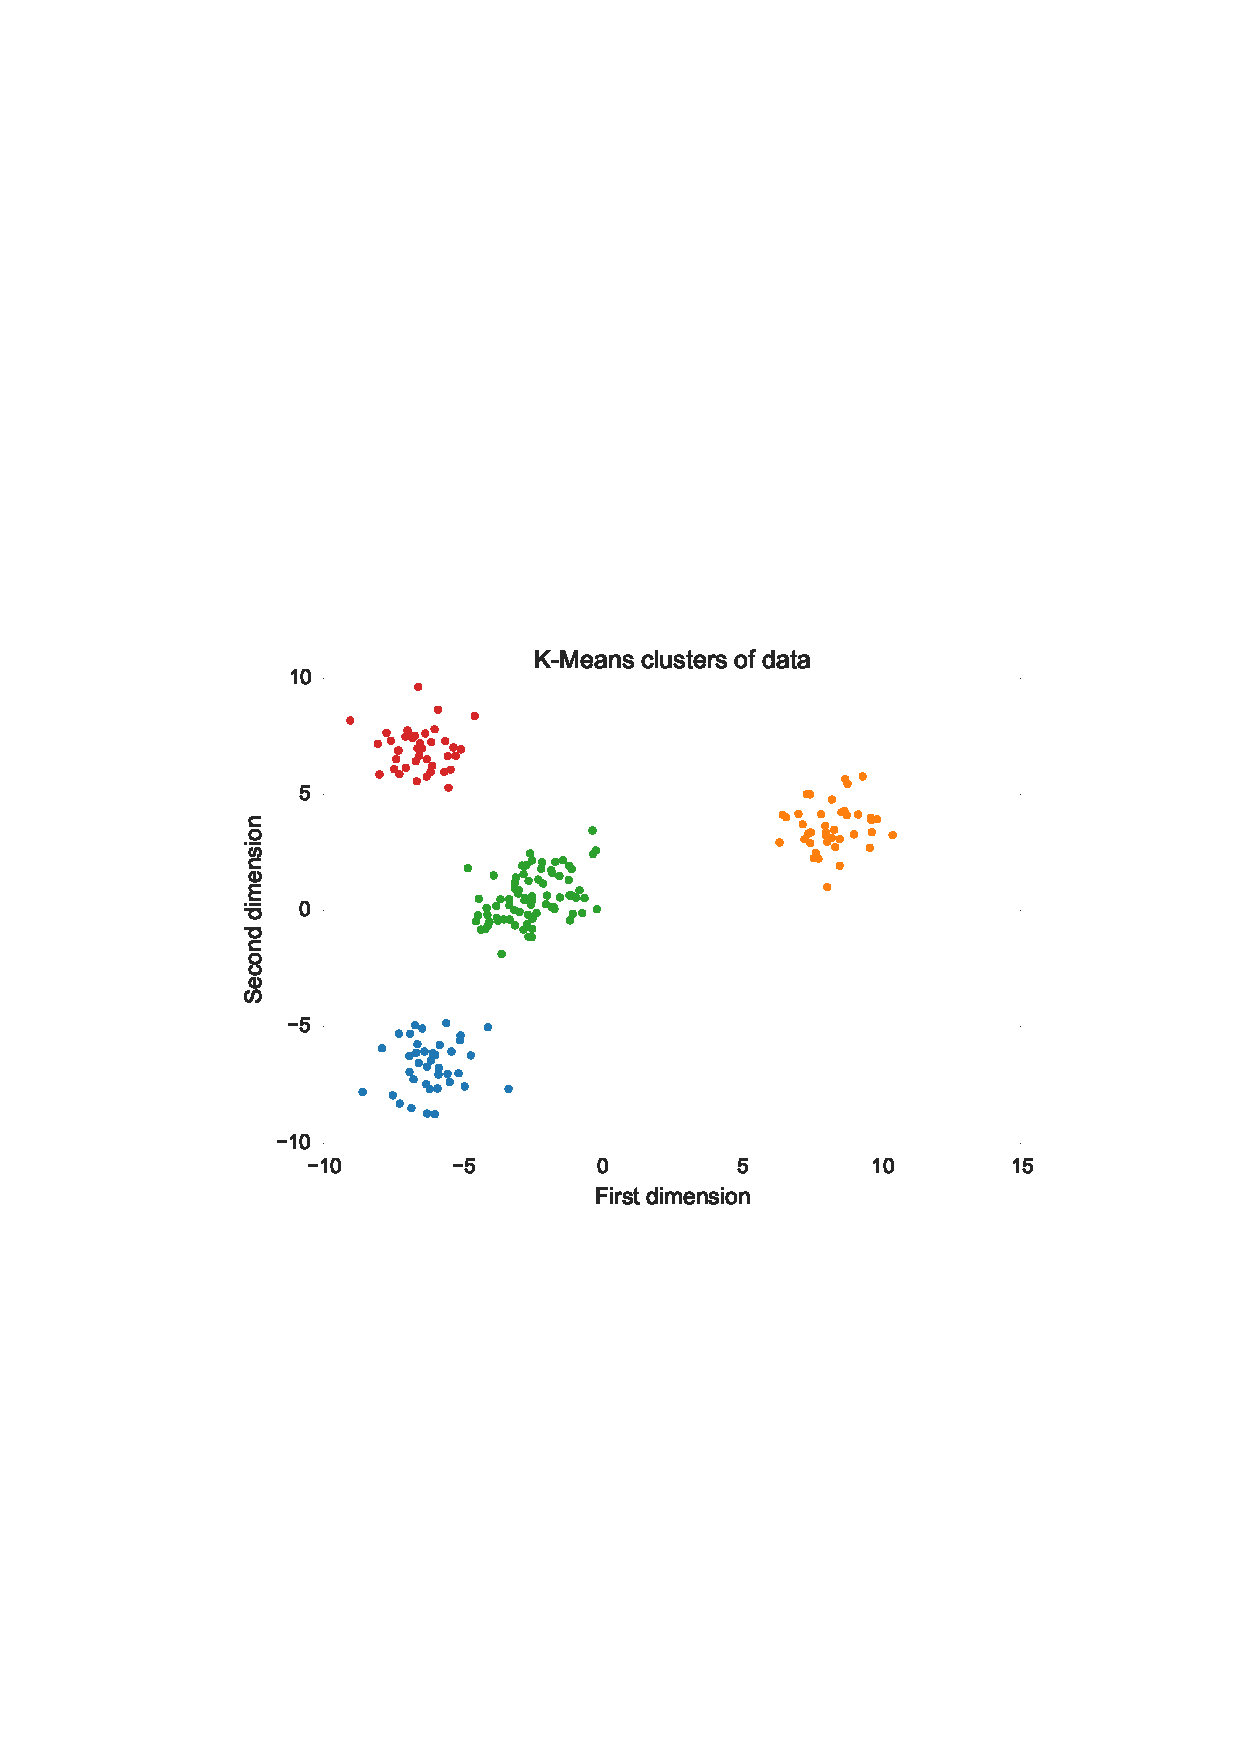
\includegraphics[width=\textwidth]{introduction/img/cluster_example_kmeans.png}
%         \caption{$y=5/x$}
%         \label{fig:five over x}
%     \end{subfigure}
%     \caption{Three simple graphs}
%     \label{fig:three graphs}
% \end{figure}

Cluster analysis is a relevant technique across several domains (\citep{Aggarwal2014}):

\begin{itemize}
	\item grouping users with similar behaviour or preferences in \textbf{customer segmentation};
	\item image segmentation in the field of \textbf{image processing};
	\item clustering gene expression data, among other application, in the domain of \textbf{biological data analysis};
	\item generation of hierarchical structure for easy access and retrieval of \textbf{information systems}; % not referenced in book
\end{itemize}

% Clustering is used in a wide variety of fields to solve numerous problems, e.g.:
% %TODO provide references to all of this
% % see https://sites.google.com/site/dataclusteringalgorithms/clustering-algorithm-applications
% % has applications with articles
% \begin{itemize}
% \item image segmentation in the field of image processing;
% \item generation of hierarchical structure for easy access and retrieval of information systems;
% \item recommender systems by grouping users by their behaviour and/or preferences;
% \item clustering customers for targeted marketing in 
% \item clustering gene expression data in biology;
% \item grouping of 
% \end{itemize}


%TODO
% problems under Big Data paradihm
% typical challenges with Big Data
% why EAC?
% combination of both
\section{Motivation}
The scope of the thesis is Big Data and Cluster Ensembles.

Success of EAC clustering on hard data sets.

Interesting problems from big data.

Combining the two.

\section{Challenges and Motivation}

\section{Goals and Contribution}

This dissertation aims to research and extend the state of the art of ensemble clustering, in what concerns the method of Evidence Accumulation Clustering and its application in large datasets, while also accessing alternative algorithmic solutions and parallelization techniques. The goal is to understand EAC's suitability for large datasets and find ways to respond to the challenges that that entails, in terms of speed and memory. In particular, an efficient parallel version for GPU of different parts of the method.

Throughout this dissertation, various clustering techniques are reviewed, implemented and tested.

\section{Objectives}
The main objectives for this work are:
\begin{itemize}

\item Review quantum inspired clustering methods

\item Study possibility of integration of quantum inspired methods in EAC

\item Review of scalability of EAC

\item Review methods and techniques designed for processing large datasets

\item Review of acceleration techniques for large datasets

\item Review of the General Purpose computing in Graphics Processing Units paradigm

\item Study possibility of integration of GPGPU in EAC

\item Devise strategies to reduce complexity of EAC

\item \textbf{Application of Evidence Accumulation Clustering in Big Data}

\item Validation of Big Data EAC on real data (ECG for emotional state discovery and/or discovery of natural groups)
\end{itemize}

\section{Outline}

Explain briefly the work done

The scope of the thesis is Big Data and Cluster Ensembles. A main requirement in this context is to have fast clustering techniques. This may be accomplished in two ways: algorithmically or with parallelization techniques. The former deals with finding faster solutions while the later takes existing solutions and optimizes them with execution speed in mind.

The initial research was under the algorithmic path. More specifically, exploring quantum inspired clustering algorithms. The findings of this exploration revealed this algorithms to be a poor match for integration in EAC and turned the focus of the research to parallelization techniques. Two main paradigms of parallelization were found appropriate: GPGPU and distributed (among a cluster of workstations). While the first is a readily available resource in common machines, the second is able to address problems dealing with larger datasets.

